\documentclass[italian, twoside]{sapthesis} %remove "english" for a thesis written in Italian
%Bachelor's (laurea triennale) thesis : Lau 
%Master's (laurea specialistica) thesis: LaM 
%PhD's thesis: PhD 
\usepackage[italian]{babel} %use this package for a thesis written in Italian
\usepackage[utf8]{inputenx}
\usepackage{indentfirst}
\usepackage{microtype}
%\usepackage{chemformula}
%\usepackage{setspace}
%\usepackage{yfonts,color}
%\usepackage{siunitx}
%\usepackage{comment}
%\usepackage{multirow}
%\usepackage{varioref}
%\usepackage[bottom]{footmisc}
%\usepackage{wrapfig}
\usepackage{float}
%\usepackage{type1cm}
\usepackage{lettrine}
\linespread{1.25} %1.25*1.2 = 1.5 (MSWord linespacing)
\usepackage{chngcntr}
\usepackage[nottoc, notlof, notlot]{tocbibind}
%\onehalfspacing
\counterwithout{footnote}{chapter}
\usepackage{hyperref}
\usepackage{listings}
\usepackage{color}
\definecolor{dkgreen}{rgb}{0,0.6,0}
\definecolor{gray}{rgb}{0.5,0.5,0.5}
\definecolor{mauve}{rgb}{0.58,0,0.82}
\lstset{frame=tb,
  language=Python,
  aboveskip=3mm,
  belowskip=3mm,
  showstringspaces=false,
  columns=flexible,
  basicstyle={\small\ttfamily},
  numbers=none,
  numberstyle=\tiny\color{gray},
  keywordstyle=\color{blue},
  commentstyle=\color{dkgreen},
  stringstyle=\color{mauve},
  breaklines=true,
  breakatwhitespace=true,
  tabsize=3
}
\hypersetup{
			colorlinks=true,
			linkcolor=red,
            linktoc=page,
			anchorcolor=black,
			citecolor=red,
			urlcolor=blue,
			pdftitle={Gestione di reception mediante robot mobili},
			pdfauthor={Giovanni Magliocchetti},
			pdfkeywords={thesis, sapienza, roma, rome, university, robot, receptionist, giovanni magliocchetti, magliocchetti}
 }
% \setlength{\headheight}{25.33461pt}
% \addtolength{\topmargin}{-11.7346pt}
\title{Gestione di reception mediante robot mobili}
\author{Giovanni Magliocchetti}
\IDnumber{1896778}
\course{Ingegneria Informatica e Automatica}
\courseorganizer{Dipartimento di Ingegneria Informatica, Automatica e Gestionale}
\submitdate{2021/2022}
\copyyear{2022}
\advisor{Prof. Luca Iocchi}
\authoremail{magliocchetti.1896778@studenti.uniroma1.it}
% \examdate{12 December 2022}
% \examiner{Prof. ...} \examiner{Prof. ...} \examiner{Prof. ...}  \examiner{Prof. ...}  \examiner{Prof. ...} \examiner{Prof. ...}  \examiner{Prof. ...}

\begin{document}

\frontmatter
\maketitle

\begin{abstract}
Questa relazione tratta della programmazione di robot mobili per la realizzazione del Task numero 3 "Receptionist" della RoboCup@Home Education Challenge 2022. In sette capitoli: introduzione della competizione, presentazione del robot, spiegazione del task e dei problemi affrontati, implementazione della soluzione, riflessioni su possibili migliorie e conclusioni.
\end{abstract}

\tableofcontents

\mainmatter
\chapter{Introduzione}
\lettrine[lines=2, findent=3pt, nindent=0pt]{Q}{}uesta relazione parlerà del tirocinio svolto con il Professor Luca Iocchi del Dipartimento di Ingegneria Informatica, Automatica e Gestionale (DIAG). L'argomento trattato è la programmazione di robot mobili ed in particolare è stato scelto un task dalla RoboCup@Home Education Challenge 2022. L'obbiettivo è stato quello di programmare un robot affinché soddisfacesse i requisiti per partecipare a questa competizione, attraverso lo svolgimento di uno dei tre task previsti dal Rulebook 2022. Il robot mi è stato fornito dal DIAG e dalla Robotics 3D, dunque non mi sono dovuto occupare né dell'assemblaggio né della scelta dei componenti. Per quanto riguarda la parte software, il robot è basato su MARRtino, una piattaforma basata su ROS, che mi ha permesso di programmarlo ad alto livello.

\bigskip
Nel \hyperref[chap:1]{Capitolo~\ref*{chap:1}} si parla della RoboCup@Home Education Challenge 2022

\bigskip
Nel \hyperref[chap:2]{Capitolo~\ref*{chap:2}} si espone la struttura di MARRtino

\bigskip
Nel \hyperref[chap:2]{Capitolo~\ref*{chap:3}} si descrive il task scelto ed i metodi utilizzati per risolverlo

\bigskip
Nel \hyperref[chap:4]{Capitolo~\ref*{chap:4}} si tratta l'implementazione del task

\bigskip
Nel \hyperref[chap:5]{Capitolo~\ref*{chap:5}} si riflette su possibili migliorie

\chapter{RoboCup@Home Education Challenge 2022}
\label{chap:1} 
\lettrine[lines=2, findent=3pt, nindent=0pt]{L}{}a RoboCup@Home Education Challenge è una piattaforma di competizione educativa per coltivare squadre di principianti per le sfide di RoboCup@Home e lo sviluppo di robot di servizio. Lo scopo della Sfida Educativa è aprire la partecipazione a tutti, non solo agli studenti universitari tecnici, ma anche agli studenti delle scuole superiori inesperti e al grande pubblico. L'esclusivo formato Workshop + Competizione stimola efficacemente i partecipanti alle prime armi per lo sviluppo di robot di servizio impegnativi e l'apprendimento dell'Intelligenza Artificiale durante il tempo dell'evento. Essa viene ospitata a livello locale (regionale e nazionale) ed internazionale.

\begin{figure}[H]
    \centering
    \frame{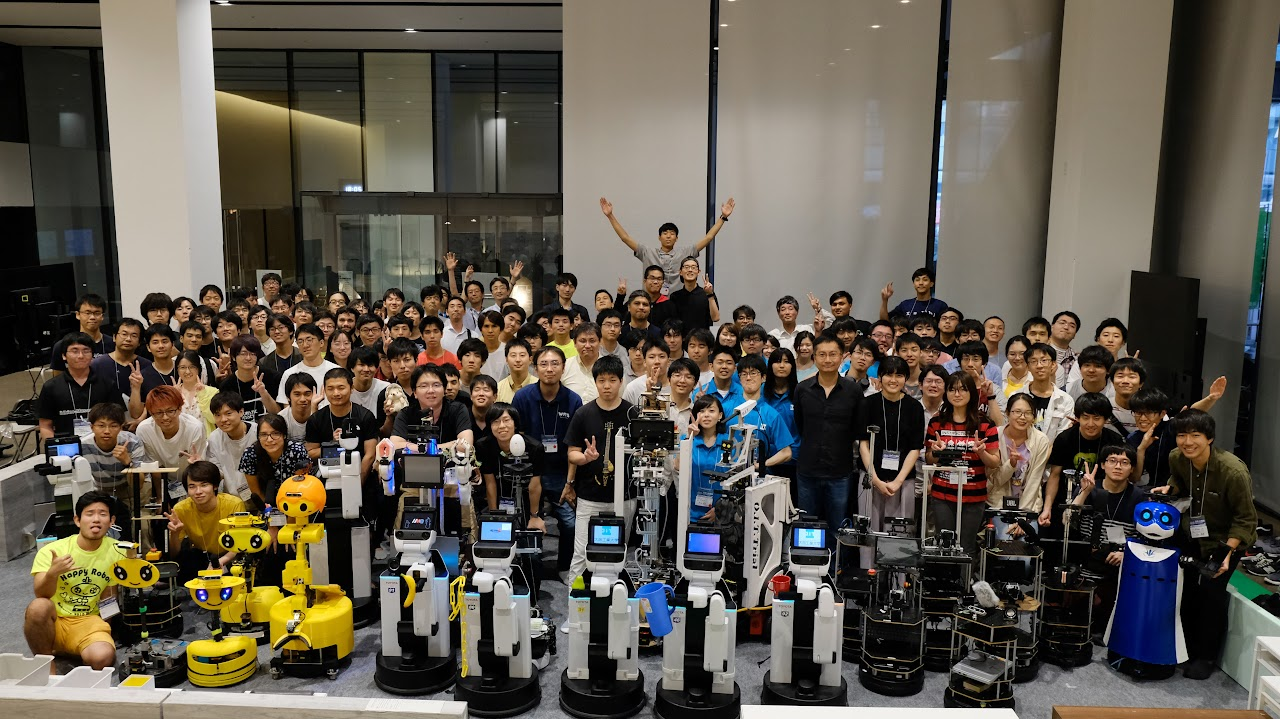
\includegraphics[width=\textwidth]{assets/robocup.jpg}}
    \caption{RoboCup@Home Education Challenge @ RoboCup Japan Open 2019.}
    \label{fig:robocup.jpg}
\end{figure}

\section{Tasks}
La challenge propone tre diversi task tra i quali è possibile scegliere quello che si vuole realizzare. I task proposti per l'edizione 2022 sono stati:

\subsection{Task 1: Carry My Luggage}
Questo task prevede che il robot rilevi una borsa, la afferri e segua un operatore umano fino alla sua automobile per poi riconsegnargli la borsa.

\subsection{Task 2: Find My Mates}
Questo task richiede di rilevare un ospite, muoversi di fronte ad egli, poi recarsi di fronte ad un altro operatore umano e comunicare a quest'ultimo la posizione precisa dell'ospite. Inoltre, deve comunicare il nome dell'ospite ed una sua descrizione.

\subsection{Task 3: Receptionist}
Questo task vede il robot che intraprende un dialogo con un ospite, chiedendogli nome e drink preferito. In seguito, il robot dovrà comunicare le informazioni ottenute ad un operatore umano. Infine, il robot dovrà accompagnare l'ospite verso un posto a sedere vuoto.

\section{Scelta del task}
La scelta è ricaduta sull'ultimo task, quello del robot receptionist. La prima proposta era più appropriata per un robot che fosse dotato di un braccio meccanico ed il robot in dotazione non ne disponeva; la seconda consisteva quasi soltanto nel riconoscere gli ospiti; il terzo task invece mi è sembrato molto più interessante e formativo, comprendendo l'utilizzo sia di funzioni di speech recognition, di mapping e navigation e di computer vision (in particolare face recognition).

\chapter{MARRtino}
\label{chap:2}
\lettrine[lines=2, findent=3pt, nindent=0pt]{M}{}ARRtino è una piattaforma robotica a trasmissione differenziale a basso costo basata su ROS, disponibile in molte forme. È stato progettato per essere facile da costruire e facile da programmare, ma allo stesso tempo utilizza software professionali basati su ROS. È quindi adatto per implementare e sperimentare molti compiti tipici della Robotica e dell'Intelligenza Artificiale, come la navigazione intelligente, l'interazione vocale uomo-robot, l'analisi delle immagini e molto altro. MARRtino viene utilizzato con successo in una varietà di attività educative, che vanno dai bambini in età prescolare al PhD e PostDoc in Intelligenza Artificiale e Robotica.

\section{Componenti hardware}
\begin{figure}[H]
    \centering
    \frame{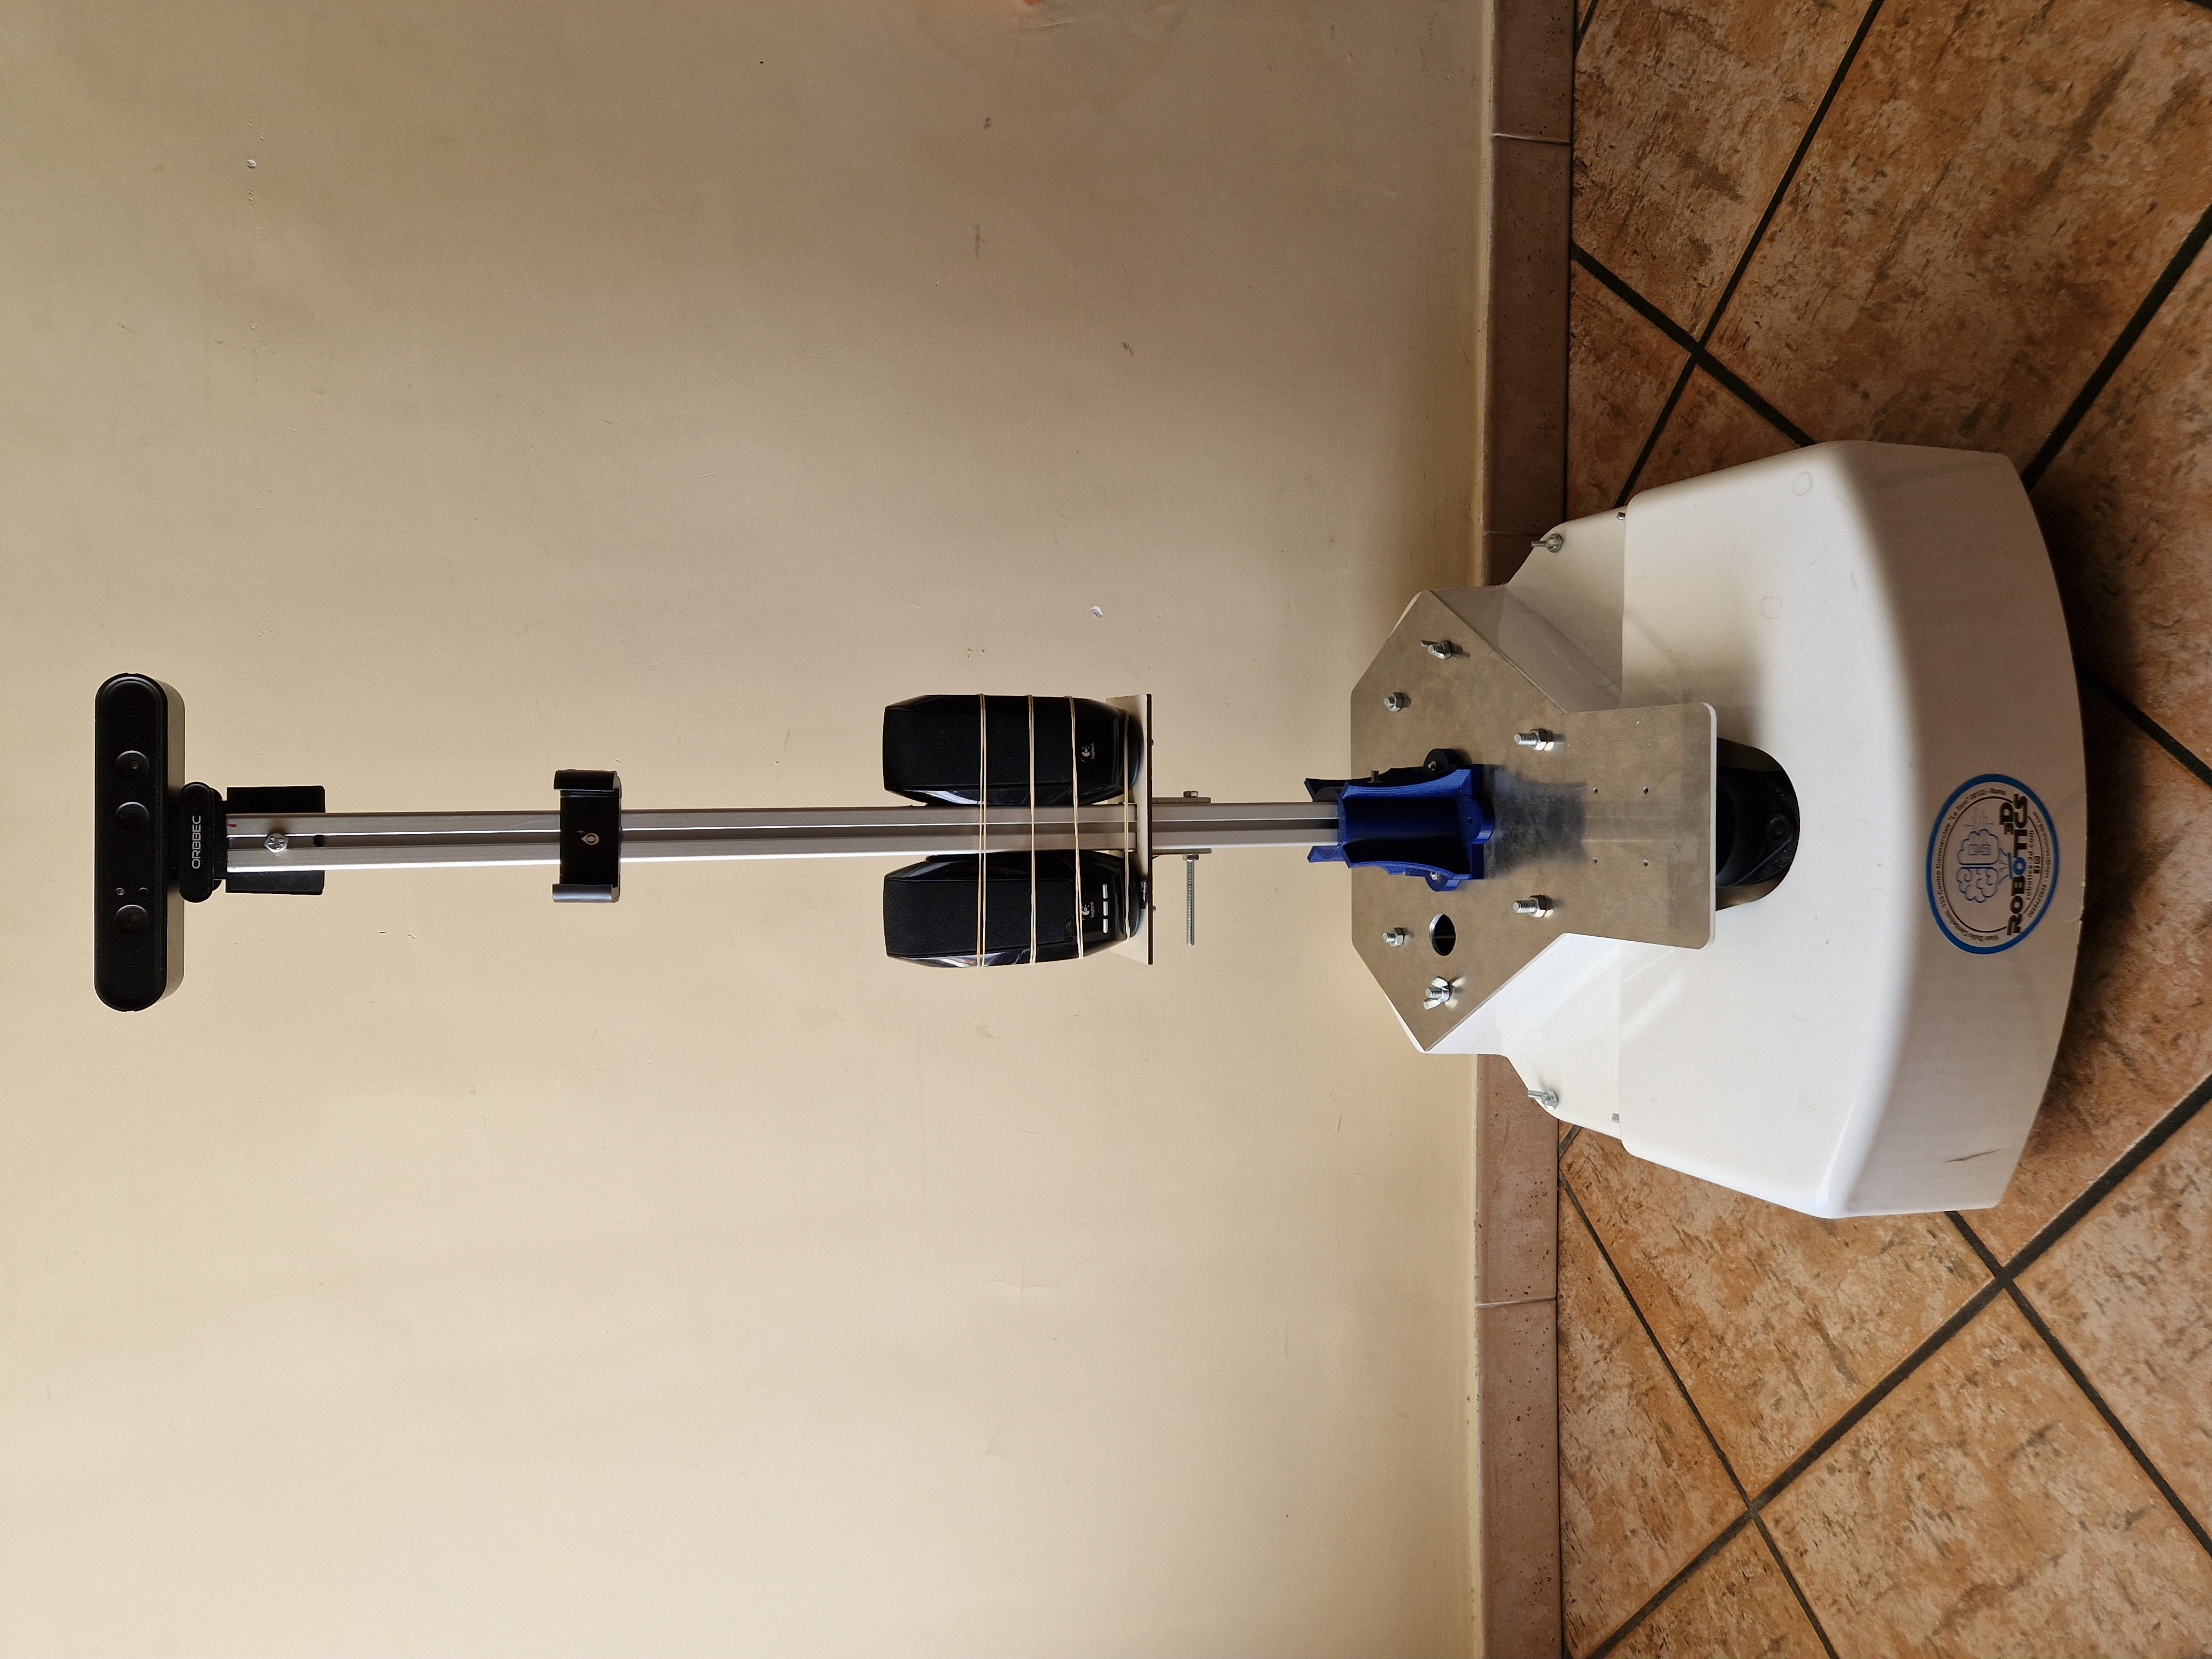
\includegraphics[angle=-90,width=0.75\textwidth]{assets/robot.jpg}}
    \caption{Esemplare di robot utilizzato}
    \label{fig:robot}
\end{figure}

Il robot utilizzato per lo svolgimento di questo tirocinio è stato gentilmente fornito dal DIAG e da Robotics 3D. Come si può notare dalla \hyperref[fig:robot]{Figura~\ref*{fig:robot}}, questo particolare esemplare è composto da:

\begin{itemize}
	\item quattro ruote (di cui due motrici) per muoversi;
	\item una videocamera ASTRA per la cattura di immagini dal mondo esterno;
	\item un sistema di altoparlanti stereo per poter "parlare" con utenti esterni attraverso il Text-To-Speech (TTS).
\end{itemize}

Per quanto riguarda la parte di STT (Speech-To-Text), ovvero ciò che permette ad un utente esterno di parlare con il robot, si può notare che l'esemplare in questione non ha incorporato alcun "microfono". Questo perché la comunicazione "da umano a robot" avviene attraverso l'apposita applicazione per smartphone Android. Essa si avvale dell'oramai molto affidabile riconoscimento vocale di Google per sintetizzare e convertire in testo l'input vocale dell'utente, per poi essere inviato al robot per l'elaborazione.

\section{Componenti software}
Ciò che caratterizza MARRtino è proprio la semplicità con cui è possibile interagire con il nostro robot, e vengono messe a disposizione diverse opzioni:

\begin{itemize}
	\item senza installazione (script Python via web browser web o VNC);
	\item macchina virtuale MARRtino (con VirtualBox);
	\item qualsiasi distribuzione Linux, fornita di Docker, Docker-Compose e marrtinoapps.
\end{itemize}

Durante i primi giorni ho utilizzato la macchina virtuale MARRtino, essendo lo strumento consigliato per avere un'esperienza già pre-configurata. Durante la mia attività di tirocinio, però, sono stati effettuati numerosi aggiornamenti volti a containerizzare il più possibile gli strumenti messi a disposizione. Ciò mi ha permesso di migrare, dopo aver adeguatamente compreso come utilizzare tali strumenti, verso la terza opzione. Nello specifico, ho utilizzato una distribuzione Ubuntu tramite il Sottosistema Windows per Linux (WSL), che fornisce prestazioni nettamente migliori rispetto alla più classica virtualizzazione con VirtualBox.

\subsection{marrtinoapps}
Il cuore di MARRtino sono le marrtinoapps. Esse mettono a disposizione dei container Docker che lavorano tra loro per permetterci di interagire con il nostro robot:
\subsubsection{Teleop}
Componente che ci permette di telecomandare il robot con l'ausilio di un joystick o della tastiera. Essa ci permette inoltre di scegliere se avvalerci o meno dell'evitamento degli ostacoli (obstacle avoidance).
\subsubsection{Camera}
Questa componente fa uso della sola videocamera per recuperare immagini dal
mondo reale. Le funzioni di questo modulo permettono non solo di controllarla,
ma danno anche la possibilità di lavorare su object recognition e face recognition.
Purtroppo quest'ultima parte è poco sviluppata a causa della grande potenza
di calcolo richiesta per eseguire queste operazioni.
\subsubsection{Laser}
Componente deputata alla gestione del sensore laser, necessario per l'obstacle avoidance e per il calcolo della distanza/profondità.
\subsubsection{Audio}
Server audio che si occupa del dialogo tra robot e umano.
\subsubsection{Stage}
Nel caso non si disponga di un robot fisico, è possibile avvalersi della simulazione 2D.
\subsubsection{Marker}
Rilevazione di AprilTags.
\subsubsection{Navigation}
Componente che gestisce lo spostamento nello spazio e l'obstacle avoidance. Lavora a stretto giro con la componente di mapping.
\subsubsection{Mapping}
Componente che ci permette di mappare l'ambiente, ad esempio la nostra casa. In questo modo possiamo ordinare al robot di andare in un determinato punto specificando le sue coordinate. Il robot effettua la mappatura in combinazione con la componente di navigation.
\section{Interazione software-hardware}
Il robot, all'accensione, espone un server accessibile collegandosi al suo access point Wi-Fi. Una volta connessi, possiamo avviare manualmente i singoli componenti o configurare un più conveniente script di autostart, per avviare le componenti che necessitiamo utilizzare in modo automatizzato. Inoltre, collegandoci via SSH all'indirizzo statico 10.3.1.1 (utente "marrtino") possiamo accedere a tutto ciò che è presente sul NUC del robot, scaricare gli aggiornamenti più recenti o apportare modifiche di qualsiasi tipo. Una volta avviato l'ambiente MARRtino, possiamo finalmente dedicarci all'attività di programmazione del robot.

\begin{figure}[H]
    \centering
    \frame{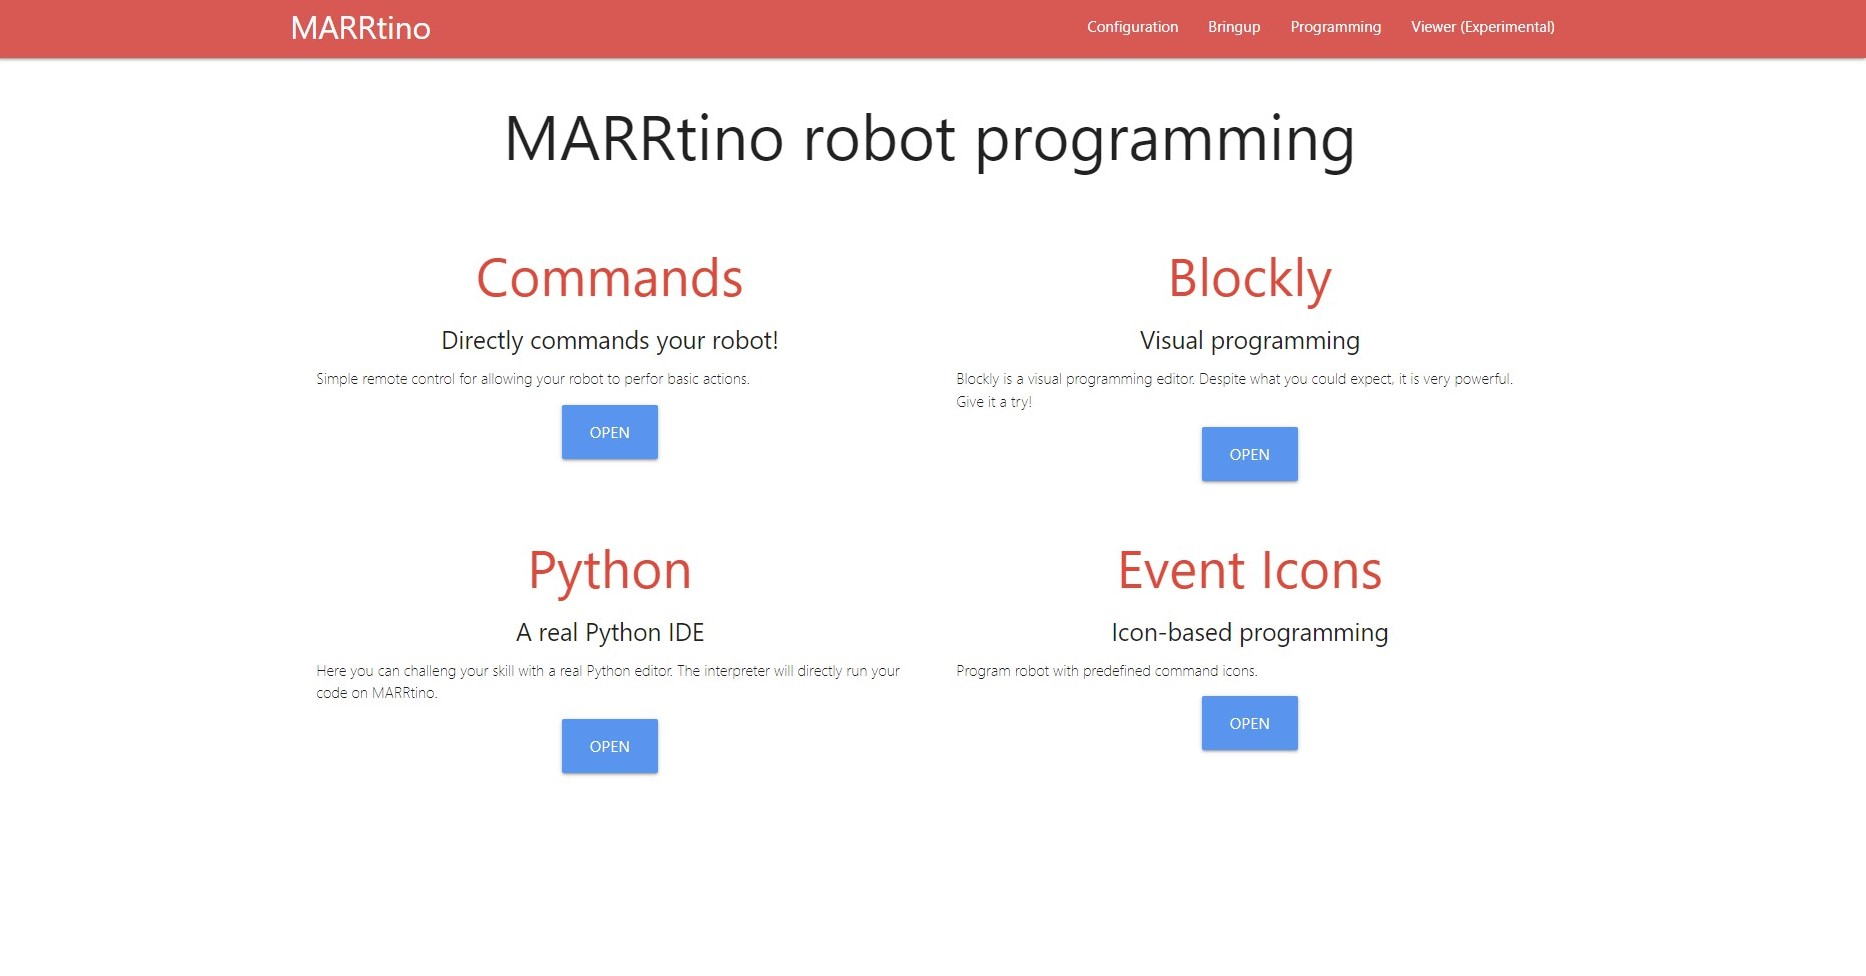
\includegraphics[width=\textwidth]{assets/marrtinoprogramming.jpg}}
    \caption{Interfaccia web MARRtino, sezione Programming}
    \label{fig:marrtinoprogramming}
\end{figure}

Come si può notare dalla \hyperref[fig:marrtinoprogramming]{Figura~\ref*{fig:marrtinoprogramming}}, per programmare il robot è possibile scegliere tra tre modalità:

\subsection{Programmazione ad icone}
Programmazione del robot con delle icone cliccabili. E' una modalità molto limitata, prevede infatti solo comandi basilari di movimento (avanti, indietro, destra e sinistra) e di riproduzione di suoni.
\subsection{Programmazione Blockly}
Programmazione del robot con dei blocchi di codice che rappresentano singole funzioni. Rappresentati come pezzi di puzzle, possono essere trascinati ed uniti tra loro grazie ad un'interfaccia grafica molto user-friendly. In questo modo si permette di programmare il robot anche a persone che non possiedono particolari skill di coding.
\subsection{Programmazione Python}
Programmazione del robot con Python, per mezzo di semplici funzioni. Ad esempio, la funzione forward(x) fa compiere x passi in avanti al robot; la funzione say(text, language) fa pronunciare al robot una frase in una lingua a nostra scelta; la funzione goto(x,y,th) ordina al robot di spostarsi nelle coordinate specificate. E' possibile programmare in Python sia eseguendo il codice nell'interfaccia web che all'interno del robot tramite l'ambiente SSH citato precedentemente.

\chapter{Robot receptionist}
\label{chap:3}
\lettrine[lines=2, findent=3pt, nindent=0pt]{I}{}n questo capitolo verrà trattato il task nella sua interezza, affrontando i suoi sottotask ed i problemi che presentano, spiegando poi alcuni dei metodi utilizzati per risolverli. Dunque, non verrà trattata l'implementazione pratica del task (che invece vedremo nel \hyperref[chap:4]{Capitolo~\ref*{chap:4}}), ma verranno elaborati in linea teorica i temi affrontati. Il task scelto per questo tirocinio è il task numero 3 della RoboCup@Home Education Challenge 2022. Esso presenta i seguenti sottotask:

\begin{itemize}
	\item presentare il primo ospite a John
	\begin{itemize}
	    \item comunicare il nome del primo ospite;
	    \item comunicare il drink preferito del primo ospite;
	    \item guardare il primo ospite mentre lo si sta introducendo.
    \end{itemize}
	\item offrire al primo ospite un posto a sedere
	\begin{itemize}
	    \item rilevare un posto vuoto;
	    \item guardare il posto vuoto mentre lo si offre.
    \end{itemize}
% 	\item BONUS: offrire agli anziani un posto a sedere su un sofà
\end{itemize}

I sottotask non rispetteranno questa suddivisione, ma verranno raggruppati per tema e problemi riscontrati, in modo da accorpare azioni simili ed evidenziare gli ostacoli affrontati nel lavoro.

\section{Comunicazione con l'ospite e problema di face detection and recognition}
La prima cosa che viene richiesta dal task è parlare con l'ospite. Infatti, per poterlo presentare all'operatore umano è necessario prima conoscerlo, il che implica l’averci parlato in precedenza. Tuttavia, prima ancora di interagire con l’ospite bisogna riconoscerlo (cioè sapere chi è un ospite e che caratteristiche ha). In altre parole, il robot deve poterlo distinguere dal resto dell’ambiente. Qui si presentano due possibili problemi a seconda del livello di raffinatezza che deve avere il task. Se si vuole che il robot riconosca semplicemente gli ospiti, ignorando le loro differenze, bisognerà affrontare un problema di face detection. Se invece si desidera che il robot sia in grado di distinguere i diversi ospiti, ci si dovrà confrontare con un problema di face recognition. Tratteremo questi due problemi in sottosezioni separate poiché nonostante sembrino simili nella teoria, nella pratica non lo sono poi così tanto.\footnote{Maggiori informazioni su questo genere di problemi si trovano nel libro Computer vision: algorithms and applications \cite{szeliski2022computer}.}.

\subsection{Face detection}
Questo primo problema tratta il riconoscimento delle facce, ovvero la capacità di saper distinguere quello che è un viso da quello che non lo è. Non importa dunque chi sia il soggetto che si sta osservando, ma solo che abbia una faccia. Come categorizzato da Yang, Kriegman, e Ahuja \cite{yang2002detecting} gli approcci possibili sono tre:

\subsubsection{Feature-based}
Questa tecnica si basa sul cercare di trovare tratti distintivi di una faccia (come gli occhi, la bocca ed il naso) e verificare che questi siano in posizioni plausibili.
\subsubsection{Template-based}
Questo approccio permette il riconoscimento di una faccia anche in diverse posizioni e con varie espressioni. Richiede una buona inizializzazione con un viso il più possibile vicino alla realtà. Non fornisce però un risultato rapido.
\subsubsection{Appearence-based}
Questa soluzione consiste nello scansionare piccoli frammenti rettangolari dell’immagine sovrapposti tra loro alla ricerca di buoni candidati ad essere una faccia. Per raffinare la ricerca, a questi possono essere poi applicati a cascata altri algoritmi di face detection. Per ovviare al problema del cambio di scala, l’immagine viene convertita in una piramide di sotto-ottave e i suoi livelli vengono scansionati separatamente.

\subsection{Face recognition}
Quando si parla di face recognition si intende il problema di distinguere un viso dall’altro, ovvero essere capaci, date due facce, di dire se appartengono o no alla stessa persona. Poter utilizzare questa funzionalità è utile sia per l’identificazione che per la validazione. Cioè, dato un volto, si può determinare se si conosce quella persona e, data un’identità, si può verificare se corrisponde a chi si ha davanti. Questo problema, per quanto diverso dal precedente, vi è legato. Infatti, per poter riconoscere una faccia in un’immagine è necessario sapere se è presente e in che punto si trova. Le soluzioni sono costituite di due parti che hanno funzioni diverse: la prima si occupa della raccolta dei dati dall’immagine di un viso, la seconda usa questi ultimi per fare dei confronti con altre immagini che gli vengono fornite. Gli approcci usati per risolvere questo problema sono cambiati nel tempo.

\subsubsection{Approcci datati}
Sfruttano le distanze tra le caratteristiche salienti in un viso, ovvero misurano gli spazi tra le parti della faccia come bocca, naso e occhi. Queste distanze dovrebbero essere sufficientemente adeguate per distinguere diverse persone. Purtroppo però non sono sempre così precise e sono state sostituite dove possibile da metodi più sofisticati. Ulteriori informazioni su questo tipo di approcci sono fornite dagli studi di Fischler e Elschlager \cite{fischler1973representation} e di Yuille \cite{yuille1991deformable}.

\subsubsection{Approcci nuovi}
Si basano sul comparare immagini in livelli di grigio proiettate in sottospazi di dimensioni inferiori, chiamate eigenfaces e, congiuntamente, modellare variazioni di forma e aspetto usando active appearance models. Le eigenfaces si basano sull’osservazione, fatta per la prima volta da Kirby e Sirovich nel 1990 \cite{kirby1990application}, che un’immagine arbitraria contenente una faccia possa essere compressa e ricostruita partendo da un’immagine principale e aggiungendo un piccolo numero di immagini riconosciute e scalate. Queste ultime possono essere derivate da un insieme di immagini di allenamento usando principal component analysis (anche conosciuta come Karhunen–Loeve transform \cite{kirby1990application}). Uno dei maggiori vantaggi dell’uso delle eigenfaces è che riducono le comparazioni da fare in un immagine per riconoscere una faccia \cite{yu1994face} \cite{lemieux2002experiments}. La riconoscibilità di un volto, come mostrato dal lavoro di Rowland e Perrett (1995) \cite{rowland1995manipulating}, dipende tanto dalla forma quanto dal colore o dalla texture; i due ricercatori sono riusciti tramite l’analisi di queste variabili ad associarvi caratteristiche personali come il sesso e l’età.

\section{Comunicazione con l'ospite e problema di human-robot interaction}
Il fulcro del task si trova proprio in questa parte, il che rende la Human-Robot interaction il problema principale da risolvere. Per poter comunicare con gli umani il robot deve essere in grado di fare tre cose:
\begin{itemize}
    \item Ascoltare cosa è stato detto;
	\item Capire cosa è stato detto;
	\item Rispondere vocalmente.
\end{itemize}
Ognuna di queste parti è fondamentale e affronta tematiche diverse che verranno trattate in breve di seguito\footnote{Questi problemi sono meglio trattati nel libro Deep Learning di Ian Goodfellow, Yoshua Bengio ed Aaron Courville \cite{goodfellow2016deep}.}.

\subsubsection{Ascoltare cosa è stato detto}
Questa parte riguarda lo speech recognition, ovvero la capacità, dato un suono (una voce), di tradurlo in stringhe di testo, in modo che queste si possano analizzare per capire cosa è stato detto. Più precisamente si cerca di mappare segnali acustici, tradizionalmente prodotti dividendo l’audio in frammenti della durata di 20ms, alla corrispondente sequenza di parole pronunciata dall’interlocutore. Gran parte dei sistemi di speech recognition preprocessano l’input usando funzionalità specifiche disegnate a mano, alcuni invece utilizzano il deep learning con le sue funzioni di apprendimento da input naturale. Lo speech recognition è stato uno dei primi campi in cui sono state adoperate le reti neurali, tuttavia esse non hanno avuto grande successo fino a tempi relativamente recenti. Il robot, per far fronte a questo problema, utilizza l’automatic speech recognition (ASR), una funzione che cerca di creare la più probabile sequenza linguistica dato il segnale in input.

\subsubsection{Capire cosa è stato detto}
Questo è uno dei problemi più grandi per un computer, ovvero quello di comprendere il significato di una frase o di un discorso. A differenza dei linguaggi di programmazione, il linguaggio naturale non è facilmente rappresentabile da un computer, per questo esiste il Natural Language Processing. Si tratta di una branca dell’informatica che si occupa di creare sistemi in grado di comprendere il linguaggio naturale. Riuscire a capire cosa l’interlocutore sta dicendo è fondamentale per poter selezionare una risposta adeguata e passare all’ultima parte della comunicazione.

\subsubsection{Rispondere vocalmente}
Quest’ultima fase della comunicazione tratta un problema che è forse il più semplice dei tre, ovvero il text to speech. Si vuole, come dice il nome, passare da un testo alla voce in modo da permettere alla persona con cui si sta interagendo di recepire la risposta. La sintesi vocale può essere realizzata concatenando registrazioni memorizzate in un database. I vari sistemi differiscono nelle dimensioni dei campioni vocali memorizzati: un sistema che memorizza singoli fonemi o fonemi doppi permette di ottenere il numero massimo di combinazioni a discapito della chiarezza complessiva, mentre in altri, concepiti per un impiego specifico, si ricorre alla registrazione di parole intere o di intere frasi per ottenere un risultato di qualità elevata. In alternativa, un sintetizzatore può incorporare un modello dei tratti vocali e di altre caratteristiche umane per creare una voce completamente di sintesi \cite{acero2000overview}.

\section{Spostamenti e problema di SLAM}
Per poter individuare la sedia e portarci l'ospite bisogna affrontare alcuni dei principali problemi della programmazione di robot mobili. Sto parlando di navigation e mapping, queste due funzioni sono fondamentali per permettere al robot di essere autonomo negli spostamenti, senza di esse non avrebbe la consapevolezza dell’ambiente circostante e ciò renderebbe molto più difficile farlo muovere verso una determinata posizione e fargli evitare gli ostacoli. Quest’ultimo problema può comunque essere attenuato sfruttando funzioni di real time obstacle avoidance, ovvero adoperando il sensore laser del robot per rilevare gli ostacoli ogni volta che esso si sposta, e deviando il suo percorso in modo da evitarli. Un altro problema è la difficoltà nello stabilire con certezza dove si trovi il robot e come sia fatta la mappa a causa del noise presente nei dati ricavati dai sensori. Questo errore dipende appunto da quanto siano precise le rilevazioni fatte dal robot, ma anche se l’errore fosse molto piccolo nei lunghi percorsi sarebbe destinato ad accumularsi e crescere fino a impedire una navigazione corretta. I sensori che hanno questo problema non sono solo quelli per il rilevamento di ostacoli, come il sensore laser, ma anche quelli che stimano i movimenti del robot. Questi ultimi possono basarsi o sui giri delle ruote (MARRtino utilizza questo modello) oppure sulla velocità del robot e il tempo per il quale si muove. Questo problema è detto SLAM (Simultaneous Localization And Mapping) e per risolverlo molti algoritmi usano una stima probabilistica basata su diversi fattori: i rilevamenti dei sensori, le posizioni del robot stimate in precedenza e le posizioni stimate dei punti di riferimento. Per potersi orientare infatti anche il robot, come gli esseri umani, ha bisogno di punti di riferimento, che possono essere riconosciuti visivamente oppure individuati con il sensore laser, in quest’ultimo caso non si può avere la certezza di star osservando lo stesso punto. Prendendo i problemi di navigation e mapping singolarmente non si avrebbe particolare difficoltà a risolverli: se ad esempio si avesse una mappa già fatta, anche qualora lo spostamento del robot non fosse preciso, la sua posizione stimata potrebbe essere corretta verificando la distanza da determinati punti di riferimento. Tuttavia, questi due problemi dipendono l’uno dall’altro, il che rende ancora più difficile dare una stima accurata della posizione del robot e della locazione dei punti di riferimento. Gli algoritmi per risolvere SLAM procedono dunque per passi: prediction step e correction step. Nel primo si sfruttano le informazioni sull’ambiente che già si possiedono e tramite il comando di spostamento che viene eseguito, si predice la posizione del robot. Nel passo successivo si acquisiscono nuovi dati dai sensori e tramite questi si cerca di correggere la posizione sia del robot che dei punti di riferimento. Esistono vari approcci per risolvere SLAM: Kalman filter, Extended Kalman filter, Information filter, Particle filter etc. \cite{sebastian2005probabilistic}.

\section{Individuazione delle sedie e problema di object recognition}
Una parte del task richiede di indicare all'ospite una sedia vuota, si presenta quindi il problema dell’object recognition. In particolare si cerca di distinguere una sedia vuota da una occupata. Si tratta quindi nello specifico di instance recognition, ovvero si cerca di riconoscere un oggetto ben noto, magari visto da diverse angolature e con diversi sfondi. Questa differisce dal riconoscimento generale di oggetti (category-level object recognition) il quale si concentra sull’individuazione di entità appartenenti a diverse classi e risulta per questo più difficile. Nel tempo sono stati sviluppati vari metodi per l’instance recognition, alcuni usano estrarre linee, contorni o superfici 3D dalle immagini per poi confrontarle a modelli 3D di oggetti specifici, altri si concentrano sull’acquisire immagini da un grande insieme di punti di vista e illuminazioni e rappresentarle usando l’eigenspace decomposition \cite{murase1993learning}. Gli approcci più recenti tendono invece ad usare le viewpoint-invariant 2D features. Dopo aver estratto le "informative sparse 2D features" dall’immagine da confrontare e da quelle nel database, queste sono comparate a coppie e, una volta trovato un numero sufficiente di aspetti in comune, si procede con una verifica cercando una trasformazione geometrica che le allinei.\\Alcuni dei metodi più usati per l’object recognition sono basati su reti neurali, queste devono essere allenate con un adeguato set di immagini opportunamente etichettate in modo da imparare a riconoscere determinati oggetti. Ad esempio una rete neurale che deve riconoscere sedie vuote e sedie occupate deve essere addestrata su un insieme di immagini contenenti queste due classi. La qualità delle immagini e la loro quantità saranno fondamentali per generare un buon riconoscitore, questo perché la rete deve estrarre caratteristiche dalle immagini di addestramento e più queste ultime saranno vicine all’oggetto che si va ad identificare, più il sistema sarà preciso. La quantità invece è necessaria per studiare gli aspetti simili e per avere una buona varianza che permetta di individuare un oggetto anche se non è estremamente vicino alle immagini di allenamento. Un aspetto importante, specifico del task, è invece il bilanciamento del database fornito per l’addestramento, c’è infatti bisogno che la differenza tra il numero di sedie vuote e occupate non sia troppo grande, se così fosse, durante l’allenamento, la rete potrebbe trovarsi a valutare alcuni batch contenenti solo immagini di un tipo e ciò potrebbe generare un riconoscitore poco affidabile. Per evitare ciò viene usata la k-fold cross-validation \cite{bengio2003no}, la quale permette di valutare il funzionamento del riconoscitore fornendogli diversi insiemi di training data e validation data. In questo modo si può usare quello che si è dimostrato essere il migliore.

\chapter{Implementazione del task}
\label{chap:4}
\section{Ricognizione dell'ambiente esterno}
Prima di iniziare con la scrittura del codice per eseguire il task scelto, è stato necessario mappare l'ambiente in cui il robot si trovava per far sì che esso potesse ricordare i luoghi attorno a lui e raggiungerli su comando.

\begin{figure}[H]
    \centering
    \frame{\includegraphics[width=\textwidth]{assets/rviz.png}}
    \caption{Screenshot di Rviz, software per la visualizzazione della mappa.}
    \label{fig:rviz}
\end{figure}

Come è possibile vedere dalla \hyperref[fig:rviz]{Figura~\ref*{fig:rviz}}, il software Rviz ci permette di seguire in tempo reale la mappatura che il robot sta eseguendo, vedendo la mappa formarsi man mano. Dopo aver effettuato la mappatura della mia casa, ho definito delle funzioni Python che permettessero di raggiungere delle coordinate specifiche. Ad esempio, quando si invoca la funzione goToSpecificTarget("seat0"), al robot viene ordinato di posizionarsi di fronte alla prima sedia, per poter poi proseguire con il resto delle istruzioni.

\begin{lstlisting}[language=Python]
...
def goToSpecificTarget(target):
    if target == "start":
        gotoTarget(0, 0, frame='map')
    elif target == "helper":
        gotoTarget(0.1, 0.08, frame='map')
    elif target == "seat0":
        gotoTarget(1.1, 0.16, frame='map')
    elif target == "seat1":
        gotoTarget(1.1, 0.24, frame='map')
    elif target == "seat2":
        gotoTarget(1.1, 0.32, frame='map')
...
\end{lstlisting}

\section{Rilevazione del primo ospite}
Come prima cosa è stato necessario far sì che il robot rilevasse un ospite da poter interrogare. Per portare a termine ciò è stato necessario implementare all'inizio del programma un ciclo deputato a catturare un'immagine e passarla alla funzione detectMultiScale della libreria OpenCV. Tale funzione rileva oggetti di diverse dimensioni nell'immagine di input, e per il nostro scopo è stato dunque necessario fornirle anche una Haar Cascade di facce frontali. Il ciclo summenzionato viene interrotto quando viene rilevato un viso.

\begin{figure}[H]
    \centering
    \frame{\includegraphics[width=0.75\textwidth]{assets/accoglienza.jpg}}
    \caption{Accoglienza di un ospite da parte del robot.}
    \label{fig:accoglienza}
\end{figure}

\begin{lstlisting}[language=Python]
from time import sleep
import cv2

begin()

class Person:
    def __init__(self, face, name, gender, pronouns, drink):
        self.face = face
        self.name = name
        self.gender = gender
        self.pronouns = pronouns
        self.drink = drink

yes = ['yes', 'Yes', 'YES', 'Yeah', 'yeah', 'Yep', 'yep', 'YEP', 'Correct', 'correct', 'Right', 'right']
no = ['no', 'No', 'Nope', 'nope', 'Wrong', 'wrong']
maleGender = ['male', 'mail', 'man', 'men', 'boy', 'guy', 'Male', 'Mail', 'Man', 'Men', 'Boy', 'Guy']
femaleGender = ['female', 'woman', 'women', 'girl', 'gal', 'Female', 'Woman', 'Women', 'Girl', 'Gal']

# Si preleva il modello Haar Cascade per facce frontali
faceCascade = findCascadeModel()

# Funzione per prelevare l'ultima immagine catturata, in formato JPG
def getImageJPG():
    getImage()
    MARRTINO_APPS_HOME = os.getenv('MARRTINO_APPS_HOME')
    assert MARRTINO_APPS_HOME is not None
    return MARRTINO_APPS_HOME + "/www/viewer/img/lastimage.jpg"

...

faces = [] # Deve avere grandezza pari ad 1, ovvero una faccia alla volta
facesJPG = [] # Stessa condizione dell'array "faces"
guests = [] # Array con unico scopo di logging (memorizzare i profili degli ospiti)
helperName = "John" # Nome dell'helper (nel nostro caso "John")

while (faces == []):
    # Legge l'immagine catturata
    image = cv2.imread(getImageJPG(), 0)
    # Rileva le facce nell'immagine
    faces = faceCascade.detectMultiScale(
        image,
        scaleFactor=1.1,
        minNeighbors=5,
        minSize=(30, 30)
    )
    # Handler nel caso di rilevazione di due o piu' facce (vedere Paragrafo 5.2.1)
    if faces > 1:
        say("I see more than one face, please one of you step back. Will check again in 2 seconds.")
        faces = []
        sleep(2)
        continue
    # Ritaglia la faccia e la memorizza in un array
    for (x, y, w, h) in faces:
        facesJPG.append(image[y:y+h, x:x+w])
    ...
\end{lstlisting}

\subsection{Rilevazione di più di un ospite nello stesso momento}
Cosa succede nel caso venisse rilevato più di un ospite nella stessa immagine? In tal caso, sono state valutate due soluzioni:

    \begin{itemize}
	    \item il robot deve chiedere agli ospiti di posizionarsi in modo che solo un ospite alla volta venga rilevato. Il robot tornerà al punto di partenza ogni volta che termina di gestire un ospite;
	    \item il robot memorizza tutti gli ospiti rilevati e li gestisce uno alla volta.
    \end{itemize}
    
% \begin{figure}[H]
%     \centering
%     \frame{\includegraphics[width=\textwidth]{rviz.png}}
%     \caption{Caso particolare: accoglienza di molteplici ospiti.}
%     \label{fig:figura421}
% \end{figure}
    
Nonostante siano molto simili, la seconda opzione è lievemente migliore. Il problema presentatosi, però, è che, essendo l'immagine elaborata da OpenCV come una matrice, lo storing dei volti nell'array è ordinato in modo da partire dal volto più in alto a sinistra fino al volto più in basso a destra. Certamente non è fattibile chiedere agli ospiti di disporsi in un certo ordine. Ho ritenuto dunque necessario optare per la prima opzione. La differenza, come già detto in precedenza, è marginale, dato che in ambedue le soluzioni il robot gestisce un ospite alla volta. Il codice Python che gestisce questa casistica è stato già mostrato nello snippet di codice presente al Paragrafo 5.2.

\section{Comunicazione con l'ospite}
Si giunge ora ad una parte prettamente incentrata sullo speech. Tramite le funzioni say() e asr(), il robot:

\begin{itemize}
    \item chiede all'ospite il suo nome ed in seguito lo ripete chiedendo se sia corretto
    \begin{itemize}
        \item se non è corretto, viene chiesto di ripetere il nome (e viene nuovamente chiesta conferma, così via fino a quando l'ospite non ci da una risposta affermativa).
    \end{itemize}
\end{itemize}
Lo stesso procedimento si applica per le domande sul genere e sul drink preferito.

\subsection{Linguaggio gender-neutral}
Il robot porrà all'ospite anche una quarta domanda:
    \begin{itemize}
	    \item "Con quale genere ti identifichi di più?"
    \end{itemize}
Ho ritenuto questa domanda necessaria per un corretto e rispettoso utilizzo dei pronomi nei dialoghi seguenti.

\begin{lstlisting}[language=Python]
    ...
    # Mostra la faccia dell'ospite (solo su robot provvisti di display)
    display(facesJPG[0])
    # Chiede il nome dell'ospite
    name = ""
    say("Hello, what is your name?", language="en")
    nameIsCorrect = False
    while (nameIsCorrect == False):
        name = asr()
        say("Is " + name + " correct?", language="en")
        if (asr() in yes):
            nameIsCorrect = True
            name = name.capitalize()
        else:
            say("Oh, sorry, I must've heard wrong! Please repeat.", language="en")
    # Chiede il sesso dell'ospite
    gender = ""
    pronouns = ""
    say("How do you identify yourself?", language='en')
    genderIsCorrect = False
    while (genderIsCorrect == False):
        gender = asr()
        if gender in maleGender:
            say('You identify as a male, correct?', language='en')
            if (asr() in yes):
                genderIsCorrect = True
                gender = "male"
                pronouns = "he/him/his"
            else:
                say("Oh, sorry, I must've heard wrong! Please repeat.", language="en")
        elif gender in femaleGender:
            say('You identify as a female, correct?', language='en')
            if (asr() in yes):
                genderIsCorrect = True
                gender = "female"
                pronouns = "she/her/her"
            else:
                say("Oh, sorry, I must've heard wrong! Please repeat.", language="en")
        else:
            say('You identify as non-binary, correct?', language='en')
            if (asr() in yes):
                genderIsCorrect = True
                gender = "non-binary"
                pronouns = "they/them/their"
            else:
                say("Oh, sorry, I must've heard wrong! Please repeat.", language="en")
    # Chiede il drink preferito dell'ospite
    drink = ""
    say("Last question: what's your favorite drink?", language='en')
    drinkIsCorrect = False
    while (drinkIsCorrect == False):
        drink = asr()
        say("Is " + drink + " correct?", language="en")
        if (asr() in yes):
            drinkIsCorrect = True
            drink = drink.capitalize()
        else:
            say("Oh, sorry, I must've heard wrong! Please repeat.", language="en")
    # Crea un oggetto persona attraverso la classe dedicata
    person = Person(facesJPG[0], name, gender, pronouns, drink)
    # Memorizza l'oggetto persona in un array per questioni di logging
    guests.append(person)
    ...
\end{lstlisting}

\section{Raggiungimento di John}
Dopo aver memorizzato i dati dell'ospite, il robot chiede all'ospite di seguirlo per raggiungere John, grazie alla funzione integrata gotoTarget(x, y, map). Il robot è dunque al corrente dei luoghi che lo circondano grazie alla mappatura, e si ipotizza che John sia un collega umano posizionato sempre in un determinato posto. Data la mancanza di face recognition causa limitazioni hardware del robot, il robot chiederà all'ospite di rimanere sempre alla sua sinistra, in modo da sapere già dove puntare quando necessario.

\subsection{John non è presente}
Cosa succede nel caso John non fosse presente in quel momento? In tal caso, arrivato a destinazione il robot:

\begin{itemize}
    \item cattura un'immagine e controlla se in essa è presente almeno un volto
	\begin{itemize}
        \item se nessun volto è presente, dice ad alta voce di aspettare che John torni. Effettuerà un nuovo tentativo dopo 5 secondi.
    \end{itemize}
\end{itemize}

\begin{lstlisting}[language=Python]
    ...
    # Il robot va da John
    say("Okay, " + name + ", please follow me. And please always stay on my left.")
    goToSpecificTarget("helper")
    # Controlla se John e' li'
    helperIsThere = False
    while (helperIsThere == False):
        # Read the image
        image = cv2.imread(getImageJPG(), 0)
        # Detect faces in the image
        temp = faces
        faces = faceCascade.detectMultiScale(
            image,
            scaleFactor=1.1,
            minNeighbors=5,
            minSize=(30, 30)
        )
        if faces != []:
            helperIsThere = True
        else:
            say("I can't find the helper, please wait. Will check again in 5 seconds.")
            sleep(5)
        faces = temp
    ...
\end{lstlisting}

\section{Guardare l'ospite durante la sua introduzione}
Uno dei sottotask richiede che il robot guardi l'ospite mentre egli viene presentato a John. Dunque, il robot, dopo aver rilevato e salutato John, dovrà nuovamente puntare l'ospite.

\begin{figure}[H]
    \centering
    \frame{\includegraphics[width=0.75\textwidth]{assets/introduzione.jpg}}
    \caption{Introduzione dell'ospite.}
    \label{fig:introduzione}
\end{figure}

\begin{lstlisting}[language=Python]
    ...
    # Introduzione dell'ospite a John
    say("Hi " + helperName + "! This is our new guest!", language='en')
    # Trova l'ospite (per guardarlo durante l'introduzione)
    left(1)
    say(pronouns.split("/")[2] + " name is " + name + " and " + pronouns.split("/")[2] + " favorite drink is " + drink + ".", language='en')
    # Guarda John
    right(1)
    say("I'll now bring " + pronouns.split("/")
        [1] + " to an empty seat!", language='en')
    # Guarda l'ospite
    left(1)
    ...
\end{lstlisting}

\section{Rilevamento di un posto libero}
Una volta completata l'introduzione dell'ospite a John, il robot dovrà accompagnare l'ospite a sedersi. Per rilevare un posto effettivamente libero, ho fatto uso di un AprilTag. Esso è definito come un sistema fiduciale visivo, utile per un'ampia varietà di attività, tra cui realtà aumentata, robotica e calibrazione della fotocamera. I target possono essere creati da una normale stampante e il software di rilevamento AprilTag calcola la posizione 3D precisa, l'orientamento e l'identità dei tag relativi alla fotocamera.

\begin{figure}[H]
    \centering
    \frame{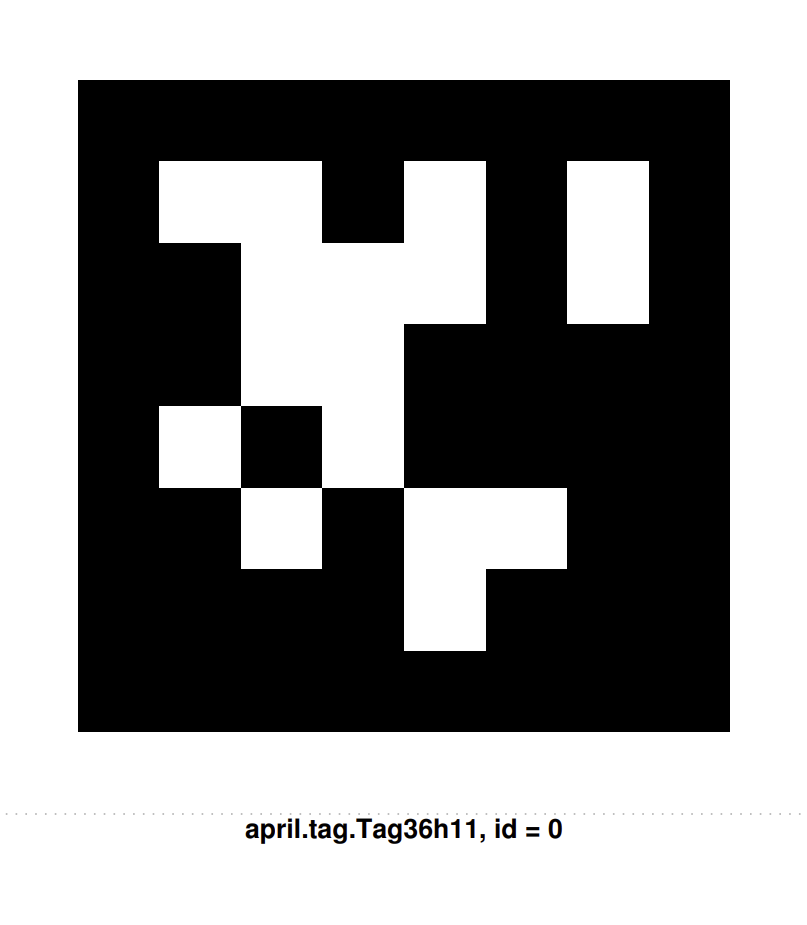
\includegraphics[width=0.75\textwidth]{assets/apriltag.png}}
    \caption{Uno dei tag riconosciuti da MARRtino.}
    \label{fig:apriltag}
\end{figure}

Nel mio caso ho utilizzato una stanza con tre sedie ed una poltrona, sullo schienale di ogni quale ho posto un foglio con un AprilTag. In questo modo, se una persona occupa un determinato posto a sedere, l'AprilTag sullo schienale è coperto (e dunque non in vista). Il robot chiederà nuovamente all'ospite di seguirlo e si recherà nella sala dei posti a sedere, nello specifico davanti alla prima sedia. A questo punto, il robot:
\begin{itemize}
    \item cattura un'immagine e controlla se in essa è presente un AprilTag
	\begin{itemize}
	    \item se è presente un AprilTag, propone all'ospite di sedersi lì;
        \item se non è presente un AprilTag, si sposta alla posizione della seconda sedia, e così via. Nel caso anche la terza ed ultima sedia risulti occupata, dirà all'ospite che purtroppo non ci sono posti liberi e che potrà attendere che qualcuno si alzi. Infine, il robot saluterà e tornerà alla posizione di partenza (per potersi occupare del prossimo ospite).
    \end{itemize}
\end{itemize}

\begin{figure}[H]
    \centering
    \frame{\includegraphics[width=0.75\textwidth]{assets/rilevazione.jpg}}
    \caption{Rilevazione posto libero tramite un AprilTag.}
    \label{fig:rilevazione}
\end{figure}

\begin{lstlisting}[language=Python]
    ...
    # Vai alla stanza dei posti a sedere
    say("Please follow me to the seats room.", language='en')
    goToSpecificTarget("seat0")
    say("There you go, " + name +
        "! Let's see if there is an empty seat for you!", language='en')
    seatPointing = "seat0"
    emptySeat = False
    while emptySeat == False:
        if tagTrigger() == True:
            emptySeat = True
            say("You can sit there! I'll go, you can find me at the reception.", language='en')
            goToSpecificTarget("start")
        if (seatPointing == "seat0"):
            goToSpecificTarget("seat1")
            seatPointing = "seat1"
        elif (seatPointing == "seat1"):
            goToSpecificTarget("seat2")
            seatPointing = "seat2"
        # se tutti i posti a sedere sono stati controllati, il robot comunichera' all'ospite che non c'e' nessun posto vuoto in quel momento
        elif (seatPointing == "seat2"):
            say("There is no empty seat at the moment. You can wait here until another guest stands up. I'll go, you can find me at the reception.", language='en')
            goToSpecificTarget("start")
            break

end()
\end{lstlisting}

% \section{BONUS: far accomodare un ospite anziano su un sofà}
% Ho deciso di cimentarmi anche nell'implementazione di una soluzione per il sottotask bonus. Questo sottotask richiedeva di far sedere un ospite anziano su di un sofà (invece di una sedia). La soluzione che ho implementato prevede che il robot:
% \begin{itemize}
%     \item faccia un check dell'età
% 	\begin{itemize}
% 	    \item se l'età dell'ospite è maggiore o uguale di 60, il robot si dirigerà verso la posizione del sofà e, sempre con il metodo dell'AprilTag, verifica se il sofà è libero
% 	    \begin{itemize}
% 			\item se il riscontro è positivo, propone all'ospite di sedersi lì
% 			\item se il riscontro è negativo, verifica se è comunque disponibile una sedia libera. Si sposta dunque alla posizione della prima sedia, e così via, seguendo lo stesso iter destinato ad ospiti under 60.
% 		\end{itemize}
%         \item se l'età dell'ospite è minore di 60, il robot adotterà il comportamento "standard" descritto nel paragrafo 4.5.
%     \end{itemize}
% \end{itemize}

% \begin{figure}[H]
%     \centering
%     \frame{\includegraphics[width=\textwidth]{rviz.png}}
%     \caption{Il robot fa accomodare un ospite anziano su un sofà.}
%     \label{fig:figura47}
% \end{figure}

\chapter{Considerazioni post-sviluppo}
\label{chap:5}
\lettrine[lines=2, findent=3pt, nindent=0pt]{N}{}el corso dello sviluppo della soluzione di questo task ho dovuto effettuare delle scelte importanti per poter soddisfare le diverse necessità del progetto, basandomi su diversi criteri, tra cui la realizzabilità di alcune implementazioni. In questo capitolo esporrò le mie riflessioni su come sia possibile non solo migliorare la soluzione al task, ma anche apportare degli enhancement per un eventuale utilizzo in un setting pratico di vita reale.

\section{Object recognition}
Per trovare una sedia libera, ho utilizzato degli AprilTags attaccati sullo schienale di ogni sedia, dato che tale tag sarebbe stato visibile dal robot solo in caso di sedia non occupata. L’altra opzione sarebbe stata l’object recognition. MARRtino dispone di funzioni deputate a questo scopo, supportate da librerie come TensorFlow. La creazione di un riconoscitore automatico di sedie, però, non è stata ritenuta fattibile dato che:
\begin{itemize}
    \item Avrebbe richiesto un egual numero di immagini di sedie vuote e di dover allenare una rete neurale;
    \item Libreria presente sul robot era molto datata (TensorFlow 1) ed aggiornarla avrebbe richiesto dei cambiamenti profondi alle marrtinoapps (le quali vengono mantenute dal Prof. Iocchi);
    \item Problemi di performance. L'hardware del robot non è idoneo a svolgere funzioni di object recognition. Per questi scopi vengono di norma utilizzati computer con caratteristiche di altissimo livello. Sarebbe pienamente possibile implementare questa soluzione connettendo il robot ad un server in grado di elaborare tali richieste da remoto, in modo da poter svolgere queste funzioni in maniera efficiente e soprattutto in tempistiche ragionevoli.
\end{itemize}

\section{Face recognition}
Quanto appena detto per l'object recognition si applica anche alla face recognition: sull'hardware del robot essa richiede molto tempo per soddisfare una singola richiesta, il che non è affatto idoneo ad un utilizzo nella vita reale. Proviamo a modificare la soluzione per soddisfare il sottotask che chiedeva di puntare l'ospite durante la sua introduzione. Invece di assumere che l'ospite è sempre alla sua sinistra, il robot, che sta guardando John, deve girare su sé stesso in senso antiorario fino ad individuare il viso dell'ospite. Considerando il caso peggiore, ovvero che l'ospite sia sulla sinistra del robot, quest'ultimo dovrà compiere ben quattro face comparison. Il tutto senza tener conto delle tempistiche necessarie alla cattura dell'immagine, altra operazione che richiede anch'essa qualche secondo di attesa. Nonostante non abbia avuto a disposizione l'hardware adatto, ho comunque scritto una versione alternativa del programma che fa uso della face recognition tramite l'omonima API per Python \cite{geitgey2017recognition}.

\section{Natural Language Processing}
Potrebbe anche essere migliorata la parte di conversazione uomo-macchina, utilizzando tecniche di Natural Language Processing (NLP) per elaborare in modo più accurato le frasi ricevute. La soluzione implementata, invece, si limita a confrontare le parole ricevute con degli array di parole predefiniti, che comprendono sia le parole precise che delle parole fuori contesto ma assonanti. Ad esempio:
\begin{lstlisting}[language=Python]
maleGender = ['male', 'mail', 'man', 'men', 'boy', 'guy']
\end{lstlisting}
In questo array notiamo che è presente la parola "mail". Questo perchè è capitato che il riconoscimento vocale da smartphone comprendesse tale parola invece di "male" a causa di una pronuncia errata della lingua inglese.

\section{Speech recognition dal robot}
Il modello di robot utilizzato è sprovvisto di un microfono, e potremmo pensare sia l'unica motivazione per cui è necessario l'utilizzo di uno smartphone Android per dialogare con il robot. In realtà, sarebbe teoricamente possibile implementare un software Python con il quale è possibile dialogare con le Speech API di Google, le stesse di cui usufruisce Android per elaborare lo Speech-To-Text. Il tutto avverrebbe grazie alle librerie Python SpeechRecognition (per eseguire il riconoscimento vocale con supporto a diversi motori ed API, online ed offline) e PyAudio (per la gestione dei canali audio, supportata anche da aziende leader come Dolby). Ovviamente, questo richiederebbe comunque la presenza di un microfono sul robot e di un account Google configurato alla fruizione delle Google Speech API.

\section{Dialogare con un database invece che con John}
Uno dei sottotask richiedeva che il robot riferisse le informazioni ad un operatore umano, John, prima di proseguire con la ricerca di un posto a sedere. Si potrebbe abbattere notevolmente il tempo necessario per gestire un ospite facendo inviare al robot i dati dell'ospite ad un server database. In questo modo il robot non avrebbe bisogno di riferire le informazioni a John e passerebbe subito alla ricerca di un posto a sedere, rendendo più efficiente il sistema per l'utilizzo in un setting di vita reale. Ancora meglio, anche i posti a sedere si potrebbero gestire tramite database, in modo che il robot verifichi subito se esiste un posto libero sul momento e gestirebbe l’ospite di conseguenza.

% \section{Metodo alternativo per riconoscere ospiti anziani}
% Il sottotask bonus chiedeva di accompagnare l'ospite anziano verso il sofà. La soluzione implementata prevede che il robot determini se un ospite si qualifica come anziano o meno in base ad un criterio di età, la quale viene esplicitamente richiesta. Un'altra soluzione potrebbe essere quella di riconoscere l'età dell'ospite in base al riconoscimento facciale. Questa metodica è affetta dagli stessi problemi descritti nei paragrafi 5.1 e 5.2, ma in questo caso si sarebbe rivelata la soluzione "peggiore". Questo perché ci sono persone anziane che potrebbero dimostrare meno anni, e ciò potrebbe ingannare il robot. In questo caso, dunque, ho ritenuto l'implementazione corrente la più corretta ed efficace.

\chapter{Conclusioni}
\label{chap:6}
\lettrine[lines=2, findent=3pt, nindent=0pt]{D}{}urante questo lavoro ho dovuto in primis impegnarmi a comprendere il funzionamento dei robot ed in particolare di MARRtino. Ho reperito tali informazioni dal sito ufficiale e, dopo aver installato ed inizializzato l'ambiente di sviluppo, ho esplorato il suo codice per comprenderne le funzioni di base. Successivamente ho affrontato il task della RoboCup@Home Education Challenge, il quale mi ha portato a ragionare su vari temi come face detection e face recognition, tag detection ed object detection, localizzazione e mapping simultanei. Alcuni di questi campi si sono rivelati molto semplici da studiare ed attuare, grazie specialmente alle funzioni di MARRtino già pronte all'uso; altri task si sono rivelati più complicati, come ad esempio la face detection e l'object recognition. Per migliorare la soluzione di questo task ci sono molti metodi, ad esempio utilizzare l'object recognition per individuare le sedie: ciò sarebbe pienamente possibile in remoto, connettendo il robot ad un server in grado di elaborare tali richieste in condizioni ottimali. Lo stesso si applica alla face recognition: nonostante sia stata implementata, essa richiede diversi secondi per soddisfare ogni richiesta, il che non è affatto idoneo ad un utilizzo nella vita reale. Potrebbe anche essere migliorata la parte di conversazione uomo-macchina, utilizzando tecniche di Natural Language Processing (NLP) per elaborare in modo più accurato le frasi ricevute. Da questo lavoro ho imparato molto su come funziona un robot, sono venuto a conoscenza di varie tecniche utilizzate per il machine learning ed ho imparato a gestire un lavoro che consiste nello sviluppo di software che necessita di interagire in tempo reale con l'hardware. In alcuni momenti mi sono trovato in difficoltà, ma ciò mi ha spronato a cercare di capire come superare gli ostacoli. Ho anche avuto modo di conoscere due laureandi (Alessandro Monteleone e Ludovico Comito) che stavano anch'essi svolgendo un task della competizione come tirocinio. Confrontarmi con loro mi è servito molto e li ringrazio di cuore. Ringrazio inoltre il Professor Iocchi che, nonostante i suoi numerosi impegni, si è sempre rivelato disponibile e pronto a chiarire qualsiasi mio dubbio con precisione e celerità. Questo progetto di tirocinio mi è servito a capire che le sfide più interessanti sono quelle più complicate, ma se vengono svolte con passione e dedizione regalano davvero tante soddisfazioni.

\backmatter
\phantomsection
% \begin{thebibliography}{17}
% \end{thebibliography}

\bibliographystyle{ieeetr}
\bibliography{refs}

\end{document}